\documentclass[letter]{article}

\usepackage{MD_estilo}

\nombre{Luna Garcés, Tomás Pérez, Pilar Vallotton y Julián Vargas.} 

\sigla{EYP290I-1} 
\curso{Series de Tiempo} 

\begin{document}
	
	\begin{pregunta}{1} 

En el presente informe se analiza la concentración de material particulado fino (MP2,5, en $\mu g _/ m^3$) medida por la estación La Florida del Sistema de Información Nacional de Calidad del Aire (SINCA, Ministerio del Medio Ambiente).La base original contiene registros diarios desde enero de 2002 hasta agosto de 2026. Para el análisis se agregaron los registros validados en promedios mensuales, obteniendo una serie de 296 observaciones. El objetivo es determinar si existen tendencia y estacionalidad en la serie, es decir, si el nivel de contaminación cambia con los años y si se repite un patrón anual, y evaluar qué tan bien pueden predecirse sus valores futuros mediante modelos de series de tiempo.
 

\section*{Datos y limpieza}

A los registros diarios de MP2,5 se le agregaron promedios mensuales utilizando únicamente los valores \textbf{validados} por el SINCA, ignorando los días sin dato, se excluyeron los registros preliminares y no validados. Por lo que de los 9.000 días disponibles, 8.304 (92,3\,\%) son los que corresponden a datos validados, lo que nos da una serie mensual de 296 observaciones entre enero de 2002 y agosto de 2026, cabe mencionar que agosto se encunetra incompleto, con un total de 22 días. Dentro de la base, Catorce meses carecen de registros validados (enero a septiembre de 2013 y enero a mayo de 2017) y  se imputaron mediante el suavizador de Kalman, que estima cada mes faltante a partir de un modelo SARIMA ajustado a la serie, usando las observaciones anteriores y posteriores, en este caso fue ajustado sobre el logaritmo de la serie con un modelo SARIMA$(1,0,0)(0,1,1)_{12}$. Se trabajó en escala logarítmica para que los valores imputados sean positivos al volver a la escala original. La Figura 1  muestra la serie con los meses imputados.

 (QUIZÁ POR TEMAS DE ESPACIO QUITAR LA FOTO) 
\begin{figure}[H]
    \centering
    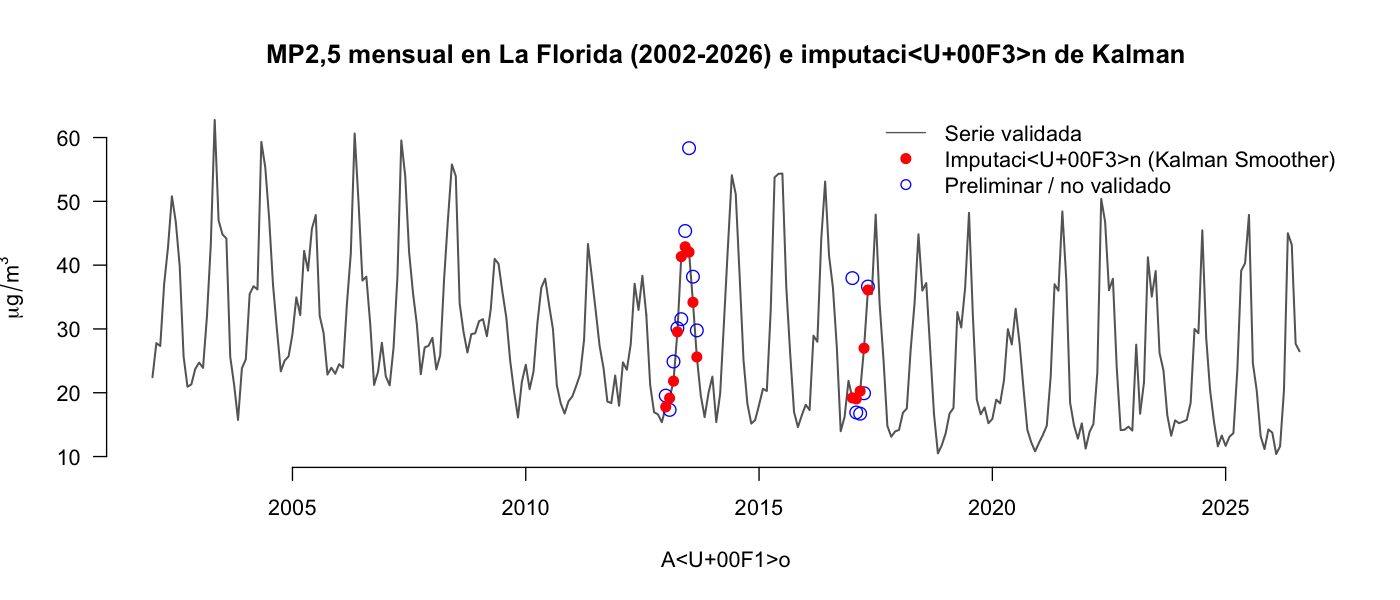
\includegraphics[width=0.75\linewidth]{fig_01.png}
    \caption{Serie mensual de MP2,5 en La Florida (2002--2026) e imputación de los meses sin datos validados.}
    \label{fig:placeholder}
\end{figure}


\section*{Análisis Exploratorio}

Al observar la serie mensual de MP2,5, se ve un patrón estacional bastante marcado, con aumentos recurrentes de contaminación durante ciertos meses del año y disminuciones posteriores. 
Además, aunque existen cambios importantes en los niveles de contaminación, no se observa una tendencia creciente durante todo el período.

Para estudiar esta estacionalidad, se analizaron la ACF, PACF y el periodograma de la serie en escala logarítmica. En la ACF se observan autocorrelaciones elevadas en los rezagos 12, 24 y 36, 
lo que indica que el comportamiento se repite aproximadamente cada año. Por su parte, la PACF presenta valores significativos en los primeros rezagos y alrededor del rezago 12.

Finalmente, el periodograma muestra un máximo cercano a $\omega=0.52$, correspondiente a un período aproximado de $2\pi/0.52 \approx 12$ meses. Por lo tanto, los resultados confirman la presencia 
de una estacionalidad anual, lo que justifica considerar modelos SARIMA para representar el comportamiento de la serie.

\begin{figure}[H]
    \centering
    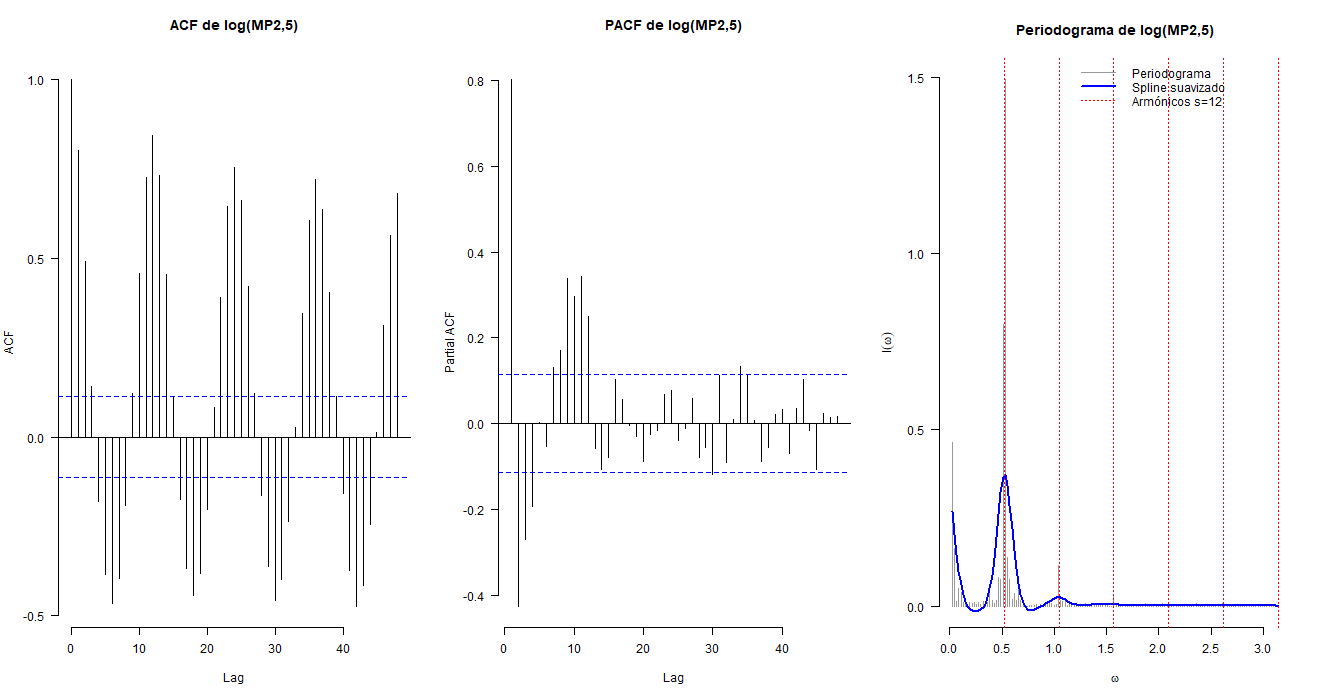
\includegraphics[width=0.92\linewidth]{fig_02.png}
    \caption{ACF, PACF y periodograma de la serie
    logarítmica de MP2,5.}
    \label{fig:exploratorio}
\end{figure}



\section*{Transformación y Estacionalidad}

Primero, se comparó el coeficiente de variación (CV) de la serie original con las transformaciones Box-Cox ($\lambda=0.20$) y logarítmica ($\lambda=0$). Se observa que la escala original presenta una mayor variación,
mientras que ambas transformaciones permiten reducirla. Sin embargo, la transformación logarítmica presenta los menores valores de CV, por lo que se decidió trabajar con $\log(X_t)$ para estabilizar la varianza.

\begin{figure}[H]
    \centering
    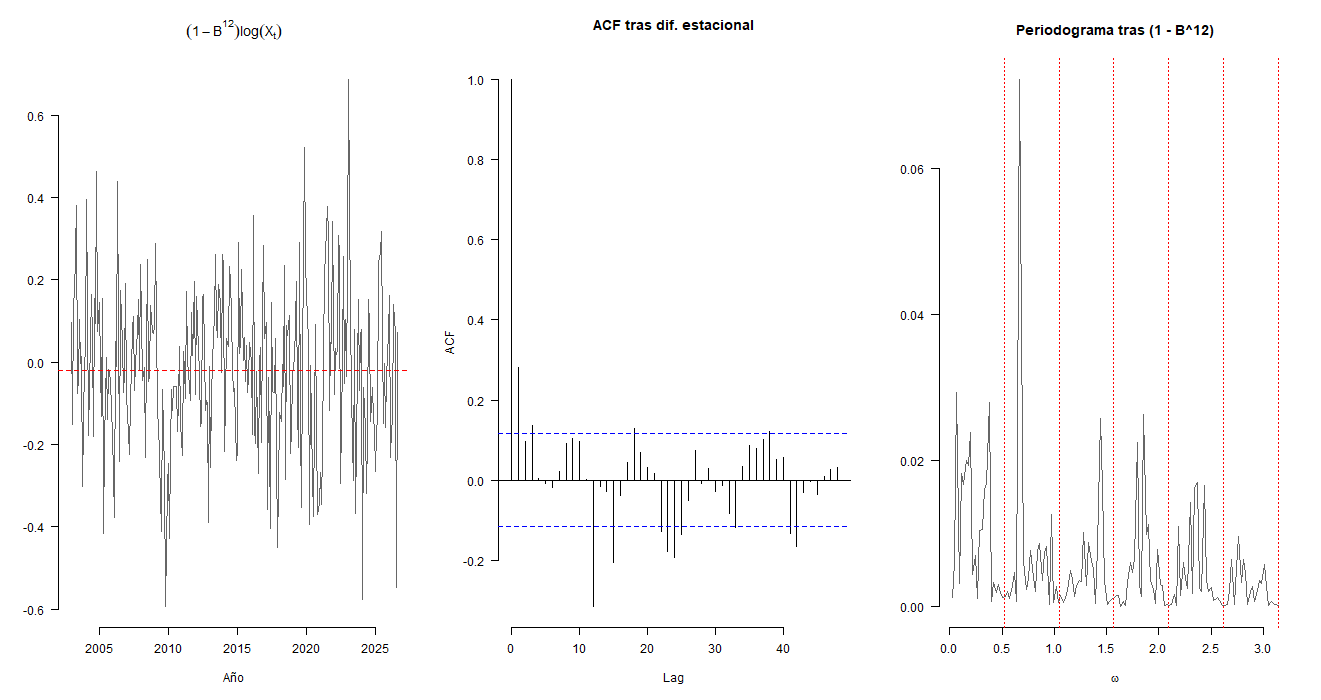
\includegraphics[width=0.85\linewidth]{fig_03.png}
    \caption{Comparación del CV anual en las tres escalas.}
    \label{fig:transformacion}
\end{figure}

Luego, para estudiar la estacionariedad, se utilizó la función \texttt{nsdiffs}, que indicó la necesidad de aplicar una diferencia estacional ($D=1$) con período 12. Por lo tanto, se trabajó con $Y_t=(1-B^{12})\log(X_t)$.
Después de aplicar esta diferencia, las pruebas \texttt{ndiffs} con ADF, KPSS y PP indicaron que no era necesaria una diferencia regular ($d=0$). Además, la prueba ADF entregó un estadístico de aproximadamente $-5.63$ y un valor-p menor a $0.01$, 
lo que permite rechazar la hipótesis de raíz unitaria.

\begin{figure}[H]
    \centering
    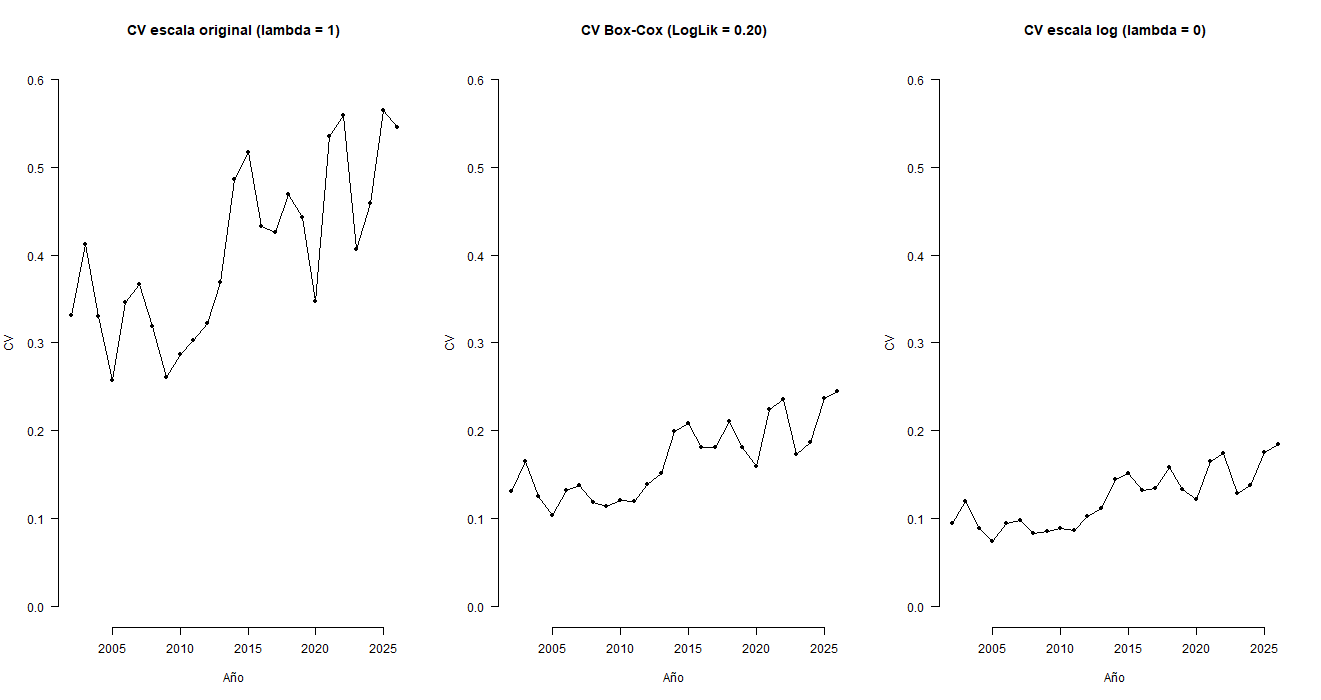
\includegraphics[width=0.85\linewidth]{fig_04.png}
    \caption{Serie, ACF y periodograma después de aplicar la diferencia estacional.}
    \label{fig:diferenciacion}
\end{figure}

Por lo tanto, se decidió trabajar con una diferencia estacional y sin diferenciación regular, es decir, con $d=0$ y $D=1$, para ajustar los modelos SARIMA.



\section*{Modelo Preliminar y Diagnósticos}

\section*{Próximos pasos}








    


\vfill

\begin{flushright}
    \textit{Gracias :)}
\end{flushright}

	\end{pregunta}

\end{document}
